\documentclass[aspectratio=169, 10pt]{beamer}

% ── Metropolis theme ──────────────────────────────────────────────────────────
\usetheme[progressbar=frametitle, block=fill, numbering=fraction]{metropolis}

% ── Custom accent colour — deep slate blue ────────────────────────────────────
\definecolor{accent}{HTML}{1F3A5F}
\definecolor{accentlight}{HTML}{EEF2F7}
\definecolor{ok}{HTML}{2E7D32}
\definecolor{warn}{HTML}{B71C1C}

\setbeamercolor{frametitle}{bg=accent, fg=white}
\setbeamercolor{progress bar}{fg=accent!70, bg=accent!20}
\setbeamercolor{alerted text}{fg=accent}
\setbeamercolor{block title}{bg=accent, fg=white}
\setbeamercolor{block body}{bg=accentlight}
\setbeamercolor{block title alerted}{bg=warn!80, fg=white}
\setbeamercolor{block body alerted}{bg=warn!8}
\setbeamercolor{block title example}{bg=ok!80, fg=white}
\setbeamercolor{block body example}{bg=ok!8}

% ── Packages ─────────────────────────────────────────────────────────────────
\usepackage{graphicx}
\usepackage{booktabs}
\usepackage{caption}
\usepackage{tikz}
\usetikzlibrary{arrows.meta, shapes.geometric, fit, positioning}
\usepackage{xcolor}
\usepackage{tabularx}
\captionsetup{font=scriptsize, skip=2pt, labelfont=bf}

% ── Convenience ──────────────────────────────────────────────────────────────
\newcommand{\hl}[1]{\textbf{\color{accent}#1}}
\newcommand{\tick}{\textcolor{ok}{$\checkmark$}}

% ─────────────────────────────────────────────────────────────────────────────
%  TITLE
% ─────────────────────────────────────────────────────────────────────────────
\title{XAI for Heart Sound Analysis}
\subtitle{RMS Review 2 --- Phase 1: Data Preprocessing Pipeline}
\author{Urva Gandhi \texttt{\small 23BCE078}\enspace|\enspace Rakshit Gajnotar \texttt{\small 23BCE077}}
\institute{B.Tech CSE, Semester 6 \quad\textbullet\quad Nirma University\\[3pt]
           Guide: Dr. Sapan Mankad\enspace\textbullet\enspace Course: RMS}
\date{3\textsuperscript{rd} April 2026}

% ─────────────────────────────────────────────────────────────────────────────
\begin{document}

% ── Title slide ───────────────────────────────────────────────────────────────
\maketitle

% ── Outline ──────────────────────────────────────────────────────────────────
\begin{frame}{Outline}
  \tableofcontents[hideallsubsections]
\end{frame}

% =============================================================================
\section{Review 1 Recap}
% =============================================================================

\begin{frame}{Review 1 --- What We Proposed}
  \begin{columns}[T]
    \column{0.50\linewidth}
      \begin{block}{Literature Review}
        \begin{itemize}
          \item Surveyed \hl{5 papers}: heart sound classification + XAI
          \item Reference: \emph{Alrabie \& Barnawi, 2025}
        \end{itemize}
      \end{block}

      \vspace{6pt}
      \begin{block}{Proposed Architecture}
        \begin{itemize}
          \item \hl{ResNet50} --- pretrained backbone
          \item \hl{SE Block} --- channel attention
          \item \hl{Multi-Head Attention} --- temporal context
          \item \hl{Grad-CAM} + \hl{SHAP} --- explainability
        \end{itemize}
      \end{block}

    \column{0.46\linewidth}
      \begin{center}
        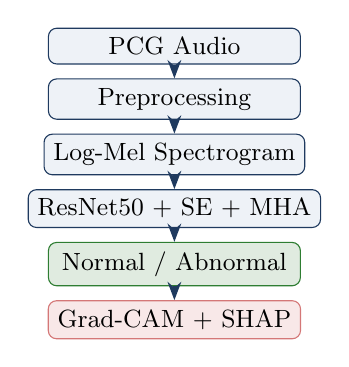
\begin{tikzpicture}[
            node distance=5pt,
            box/.style={draw=accent, fill=accentlight, rounded corners=3pt,
                        minimum width=3.2cm, minimum height=0.45cm,
                        font=\small, align=center},
            arr/.style={-Stealth, thick, color=accent}
          ]
          \node[box] (a) {PCG Audio};
          \node[box, below=of a] (b) {Preprocessing};
          \node[box, below=of b] (c) {Log-Mel Spectrogram};
          \node[box, below=of c] (d) {ResNet50 + SE + MHA};
          \node[box, below=of d, fill=ok!15, draw=ok] (e) {Normal / Abnormal};
          \node[box, below=of e, fill=warn!10, draw=warn!60] (f) {Grad-CAM + SHAP};
          \draw[arr] (a)--(b); \draw[arr] (b)--(c); \draw[arr] (c)--(d);
          \draw[arr] (d)--(e); \draw[arr] (e)--(f);
        \end{tikzpicture}
      \end{center}
  \end{columns}
\end{frame}

% =============================================================================
\section{Dataset}
% =============================================================================

\begin{frame}{Dataset --- PhysioNet CinC 2016}
  \begin{columns}[T]
    \column{0.48\linewidth}
      \begin{itemize}
        \item \hl{3,541} recordings --- training + validation
        \item Binary labels: Normal vs Abnormal
        \item Subsets: training-a to training-f + validation
        \item Variable lengths: \hl{5\,s -- 120\,s}
      \end{itemize}

      \vspace{8pt}
      \begin{alertblock}{Class Imbalance}
        \begin{tabularx}{\linewidth}{Xr}
          \textcolor{ok}{\textbf{Normal}} & 2,725\enspace (76.96\%) \\
          \textcolor{warn}{\textbf{Abnormal}} & 816\enspace (23.04\%) \\
          \midrule
          \textbf{Total} & 3,541\enspace (100\%) \\
        \end{tabularx}
      \end{alertblock}

      \vspace{6pt}
      \small Handled via \hl{class weights} in loss function.

    \column{0.50\linewidth}
      \begin{figure}
        \includegraphics[width=\linewidth]{class_distribution.png}
        \caption{Class distribution --- overall and per subset}
      \end{figure}
  \end{columns}
\end{frame}

% =============================================================================
\section{Preprocessing Pipeline}
% =============================================================================

\begin{frame}{Pipeline Overview}
  \vspace{2pt}
  \begin{center}
  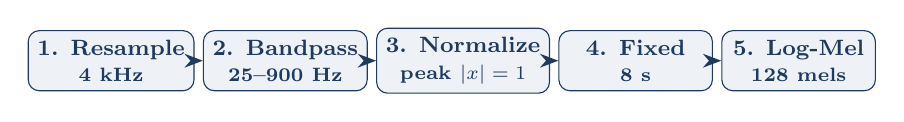
\begin{tikzpicture}[
      node distance=5pt and 3pt,
      pbox/.style={draw=accent, fill=accentlight, rounded corners=4pt,
                   minimum height=0.75cm, minimum width=1.95cm,
                   font=\footnotesize\bfseries, align=center, text=accent},
      arr/.style={-Stealth, thick, color=accent}
    ]
    \node[pbox] (s1) {1. Resample\\\scriptsize 4 kHz};
    \node[pbox, right=of s1] (s2) {2. Bandpass\\\scriptsize 25--900 Hz};
    \node[pbox, right=of s2] (s3) {3. Normalize\\\scriptsize peak $|x|=1$};
    \node[pbox, right=of s3] (s4) {4. Fixed\\\scriptsize 8 s};
    \node[pbox, right=of s4] (s5) {5. Log-Mel\\\scriptsize 128 mels};
    \draw[arr] (s1)--(s2); \draw[arr] (s2)--(s3);
    \draw[arr] (s3)--(s4); \draw[arr] (s4)--(s5);
  \end{tikzpicture}
  \end{center}

  \vspace{4pt}
  \begin{columns}[T]
    \column{0.62\linewidth}
      \begin{figure}
        \includegraphics[width=\linewidth, height=5.2cm, keepaspectratio]{preprocessing_pipeline.png}
        \caption{Raw waveform $\to$ filtered signal $\to$ Log-Mel spectrogram}
      \end{figure}
    \column{0.35\linewidth}
      \vspace{6pt}
      \begin{block}{Key Parameters}
        \begin{tabular}{ll}
          SR & 4 kHz \\
          Bandpass & 25--900 Hz \\
          Length & 8 s \\
          Mels & 128 \\
          Shape & (128, 251) \\
        \end{tabular}
      \end{block}
      \vspace{6pt}
      \small Output saved as \texttt{.npy} for fast loading.
  \end{columns}
\end{frame}

\begin{frame}{Bandpass Filter Design}
  \begin{columns}[T]
    \column{0.50\linewidth}
      \begin{figure}
        \includegraphics[width=\linewidth]{filter_response.png}
        \caption{4th-order Butterworth --- 25 to 900 Hz}
      \end{figure}

    \column{0.47\linewidth}
      \begin{exampleblock}{Bands Preserved}
        \begin{itemize}
          \item \textbf{25--150 Hz} --- S1/S2 heart sounds
          \item \textbf{150--500 Hz} --- Murmur energy
          \item \textbf{500--900 Hz} --- High-freq detail
        \end{itemize}
      \end{exampleblock}

      \vspace{8pt}
      \begin{itemize}
        \item Butterworth: flat passband, no ripple
        \item Removes baseline drift ($<$25 Hz)
        \item Removes high-freq noise ($>$900 Hz)
      \end{itemize}
  \end{columns}
\end{frame}

\begin{frame}{Why 8 Seconds? --- Duration Analysis}
  \begin{columns}[T]
    \column{0.56\linewidth}
      \begin{figure}
        \includegraphics[width=\linewidth]{duration_distribution.png}
        \caption{Recording duration distribution by class}
      \end{figure}

    \column{0.41\linewidth}
      \vspace{10pt}
      \begin{itemize}
        \item Most recordings: \hl{5--40\,s}
        \item \hl{8\,s} covers $\geq$8 heartbeats at normal HR
        \item Below median of both classes
        \item Short clips: \textbf{zero-padded}
        \item Long clips: \textbf{cropped from start}
        \item Uniform tensor shape for batching
      \end{itemize}
  \end{columns}
\end{frame}

\begin{frame}{S1/S2 Detection --- Hilbert Envelope}
  \begin{figure}
    \includegraphics[width=\linewidth, height=5.8cm, keepaspectratio]{envelope_detection.png}
    \caption{Envelope + peak detection: Normal (left) and Abnormal (right). HR $\approx$ 94--95 bpm.}
  \end{figure}
  \vspace{-4pt}
  \begin{columns}[T]
    \column{0.5\linewidth}
      \begin{itemize}
        \item Hilbert transform $\to$ analytic envelope
        \item Peaks above threshold tagged S1/S2
      \end{itemize}
    \column{0.47\linewidth}
      \begin{itemize}
        \item Consistent HR validates preprocessing
        \item \emph{Analysis only} --- not a training feature
      \end{itemize}
  \end{columns}
\end{frame}

% =============================================================================
\section{Feature Extraction \& DataLoader}
% =============================================================================

\begin{frame}{Log-Mel Spectrograms \& DataLoader}
  \begin{columns}[T]
    \column{0.54\linewidth}
      \begin{figure}
        \includegraphics[width=\linewidth]{sample_spectrograms.png}
        \caption{\textcolor{ok}{\textbf{Normal}} (top row) vs \textcolor{warn}{\textbf{Abnormal}} (bottom row)}
      \end{figure}

    \column{0.43\linewidth}
      \vspace{4pt}
      \begin{block}{Spectrogram Config}
        \begin{tabular}{ll}
          Mel bins & 128 \\
          Shape & (128, 251) \\
          Saved as & \texttt{.npy}
        \end{tabular}
      \end{block}

      \vspace{8pt}
      \begin{block}{DataLoader Config}
        \begin{tabular}{ll}
          Resize & $224 \times 224$ \\
          Channels & 3 (RGB) \\
          Normalise & ImageNet $\mu, \sigma$ \\
          Augment & SpecAugment \\
          Split & 70 / 15 / 15 \\
          Batch size & 32 \\
          Imbalance & Class weights
        \end{tabular}
      \end{block}
  \end{columns}
\end{frame}

\begin{frame}{SpecAugment --- Data Augmentation}
  \begin{figure}
    \includegraphics[width=0.84\linewidth]{augmentation_demo.png}
    \caption{Original (left) vs two SpecAugment runs --- random frequency and time masks applied}
  \end{figure}
  \begin{itemize}
    \item Randomly zeros out contiguous frequency bands and time steps
    \item Forces model to be robust to partial occlusions
    \item Applied \emph{only during training}
  \end{itemize}
\end{frame}

% =============================================================================
\section{Next Steps}
% =============================================================================

\begin{frame}{Roadmap --- Phases 2 to 6}
  \begin{columns}[T]
    \column{0.48\linewidth}
      \begin{block}{Phase 2 --- Model}
        ResNet50 + SE Block + Multi-Head Attention
      \end{block}
      \vspace{4pt}
      \begin{block}{Phase 3 --- Training}
        Frozen backbone $\to$ full fine-tune\\
        \small Weighted BCE + label smoothing
      \end{block}
      \vspace{4pt}
      \begin{block}{Phase 4 --- Evaluation}
        Accuracy $\cdot$ F1-Score $\cdot$ AUC-ROC
      \end{block}

    \column{0.48\linewidth}
      \begin{block}{Phase 5 --- XAI}
        \begin{itemize}
          \item \hl{Grad-CAM}: spatial saliency on spectrogram
          \item \hl{SHAP}: feature importance per prediction
        \end{itemize}
      \end{block}
      \vspace{4pt}
      \begin{block}{Phase 6 --- Comparison}
        Benchmark vs Alrabie \& Barnawi (2025)\\
        and other surveyed literature
      \end{block}
    \end{columns}
\end{frame}

% =============================================================================
\section*{Summary}
% =============================================================================

\begin{frame}{Summary}
  \begin{itemize}
    \setlength\itemsep{7pt}
    \item[\tick] Dataset explored --- PhysioNet CinC 2016, 3,541 recordings, imbalance identified
    \item[\tick] 5-step pipeline: resample $\to$ bandpass $\to$ normalise $\to$ fixed-length $\to$ spectrogram
    \item[\tick] Design choices validated: duration analysis, filter response, S1/S2 detection
    \item[\tick] PyTorch DataLoader: SpecAugment, class weights, stratified 70/15/15 split
    \item[\tick] 128-mel spectrograms saved as \texttt{.npy} --- ready for model training
  \end{itemize}

\end{frame}

% =============================================================================
\section*{References}
% =============================================================================

\begin{frame}{References}
\scriptsize

\begin{itemize}
\item Clifford et al., \emph{CinC}, 2016
\item Alrabie \& Barnawi, \emph{BSPC}, 2025
\item He et al., \emph{CVPR}, 2016
\item Hu et al., \emph{CVPR}, 2018
\item Vaswani et al., \emph{NeurIPS}, 2017
\item Selvaraju et al., \emph{ICCV}, 2017
\item Lundberg \& Lee, \emph{NeurIPS}, 2017
\item Park et al., \emph{Interspeech}, 2019
\end{itemize}

\end{frame}

\begin{frame}[standout]
  \Huge Thank You\\[16pt]
  \large Questions?
\end{frame}

\end{document}